\chapter{Diseño}
\label{cap:capitulo4}

\begin{flushright}
\begin{minipage}[]{9cm}
\emph{El diseño no es solo lo que se ve y lo que se siente. El diseño es cómo funciona}\\
\end{minipage}\\

Steve Jobs, \textit{conferencia de lanzamiento del Apple iPod, 2001}\\
\end{flushright}

\vspace{1cm}

Después de definir la plataforma de desarrollo, se procede a explicar el diseño de la aplicación.

El proyecto se divide en cuatro scripts, el primero se utiliza para crear o registrar un paciente, el segundo lanza la GUI y controla los parámetros del juego, el tercero permite visualizar el comportamiento del paciente durante la terapia, y el cuarto es el propio juego.

\section{Registro de un paciente}

Este script permite gestionar un conjunto de datos, que identifican a un paciente, mediante una GUI.

En primer lugar, se importan las bibliotecas estádar, mencionadas en el capítulo anterior, como \textit{tkinter}, que se utiliza para crear la interfaz gráfica, \textit{csv} para guardar los datos en un archivo .csv para su posterior uso, y \textit{os} para interactuar con el sistema de archivos.

Se obtiene el directorio de inicio del usuario y se crea un directorio dentro de este, si no existe, bajo el nombre \textit{database}, donde se almacenan los ficheros con los datos de registro y análisis terapéuticos de cada paciente.

Después, se crea una ventana principal con un título y tamaño fijo. Los datos se ingresan de forma ordenada a través de entradas de texto y hacen referencia al nombre, apellido e ID del paciente, frecuencia, amplitud y perturbación de la señal que generará el brazo robótico al inicio de la terapia, nivel y progreso del juego y un espacio para que el doctor incluya alguna observación.

Se valida que el ID sea un número, si no lo es, muestra un mensaje de advertencia.
Para guardar los datos se debe pulsar el botón \textit{Save} y para salir de la interfaz \textit{Exit}.
Los datos se guardan en un fichero .csv dentro de un subdirectorio bajo el nombre del ID. Si el archivo existe, se añaden los datos al final, si no, se crea.
Una vez los datos se han guardado, se muestra un mensaje de confirmación y se limpian los campos.
Es obligatorio especificar el ID en todos los casos, los campos restantes pueden dejarse en blanco.

En el Código \ref{cod:codejemplo}, escrito en \texttt{Python}, se muestra cómo se gestionan los directorios y la escritura del archivo .csv.

\begin{code}[h]
\begin{lstlisting}[language=Python]
def savedata():
    ID_DIR = os.path.join(DATABASE_DIR, id)
    os.makedirs(ID_DIR, exist_ok=True)
    file_name = f"{id}{ext}"
    file_path = os.path.join(ID_DIR, file_name)

    # [...]

    file_exists = os.path.isfile(file_path)
    with open(file_path, mode="a", newline="") as file:
        writer = csv.DictWriter(file, fieldnames=patient_data.keys())
        if not file_exists:
            writer.writeheader()
        writer.writerow(patient_data)
\end{lstlisting}
\caption[Función para guardar los datos de un paciente]{Función para guardar los datos de un paciente}
\label{cod:codejemplo}
\end{code}

El aspecto final de la interfaz puede observarse en la Imagen \ref{fig:database}.

\begin{figure}[ht!]
	\centering
	\begin{minipage}{0.75\linewidth}
		\centering
		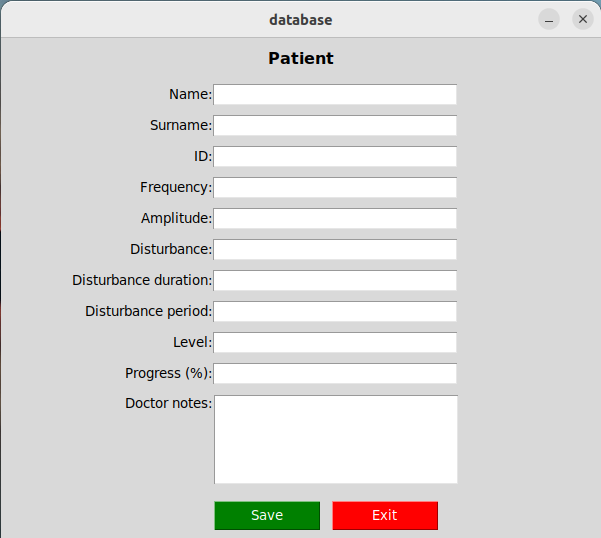
\includegraphics[width=\linewidth]{figs/registro.png}
	\end{minipage}
	\caption[Interfaz de registro de un paciente]{Interfaz de registro de un paciente}
	\label{fig:database}
\end{figure}

\section{Interfaz de control}

Este script permite especificar y controlar parámetros de una señal y perturbación para su posterior creación y uso.
Para ejecutarlo se debe especificar el archivo con los datos de registro del paciente.

Al inicio se muestra una pantalla de configuración de los límites del brazo robótico.
Para guardar la posición de mínimo y máximo, se deberá presionar el botón correspondiente, después de cada ajuste, como se observa en la Imagen \ref{fig:config}.
Para avanzar a la siguiente pantalla pulsar \textit{Continue}.

A continuación, emergerá una nueva ventana que permite ajustar la frecuencia, amplitud y offset de una señal, configurar perturbaciones especificando la intensidad, la duración y el periodo, seleccionar el tipo de señal, sinusoidal o escalón, y cambiar el nivel del juego o su dificultad.
Para actualizar estos datos se debe pulsar el botón \textit{Update signal} para las señales y \textit{Update level} para el nivel del juego.
Además, la nueva configuración se almacenará en un archivo .csv, en un subdirectorio bajo el nombre \textit{config}.

Para salir de la interfaz pulse \textit{Exit}.

En la Imagen \ref{fig:control} se muestran los campos de la segunda ventana.

\begin{figure}[ht!]
	\centering
	\begin{minipage}{0.85\linewidth}
		\centering
		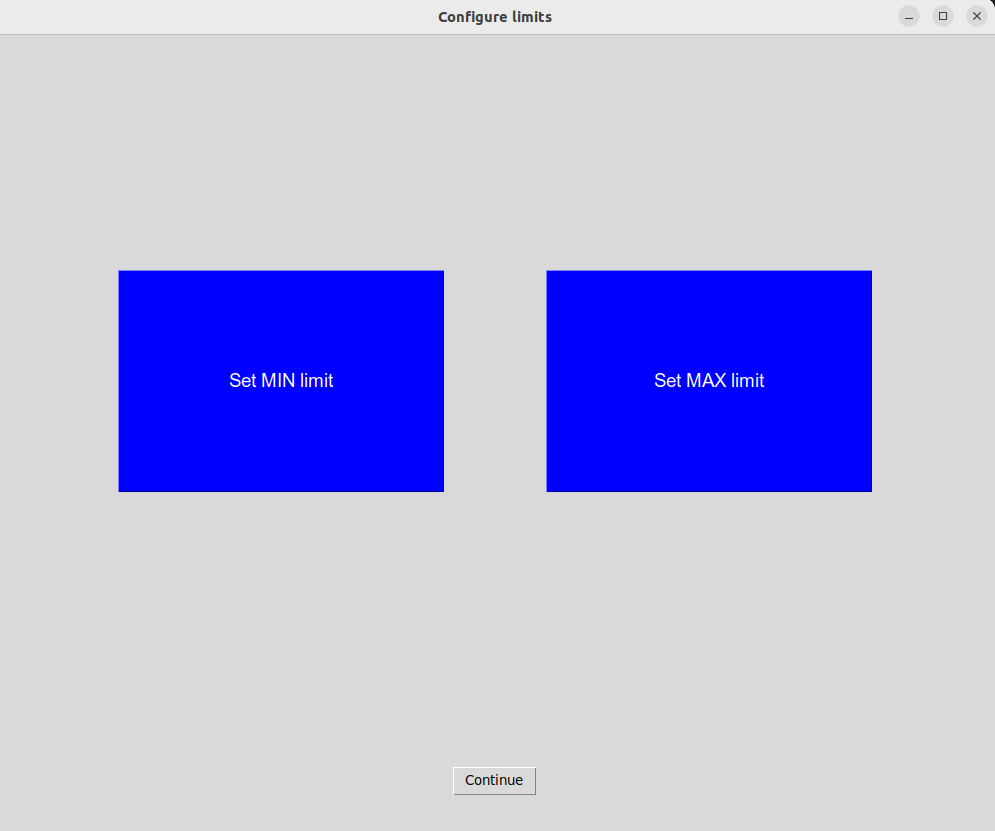
\includegraphics[width=\linewidth]{figs/config_limits.png}
	\end{minipage}
	\caption[Interfaz de configuración de los límites del brazo robótico]{Interfaz de configuración de los límites del brazo robótico}
	\label{fig:config}
\end{figure}

\begin{figure}[ht!]
	\centering
	\begin{minipage}{0.85\linewidth}
		\centering
		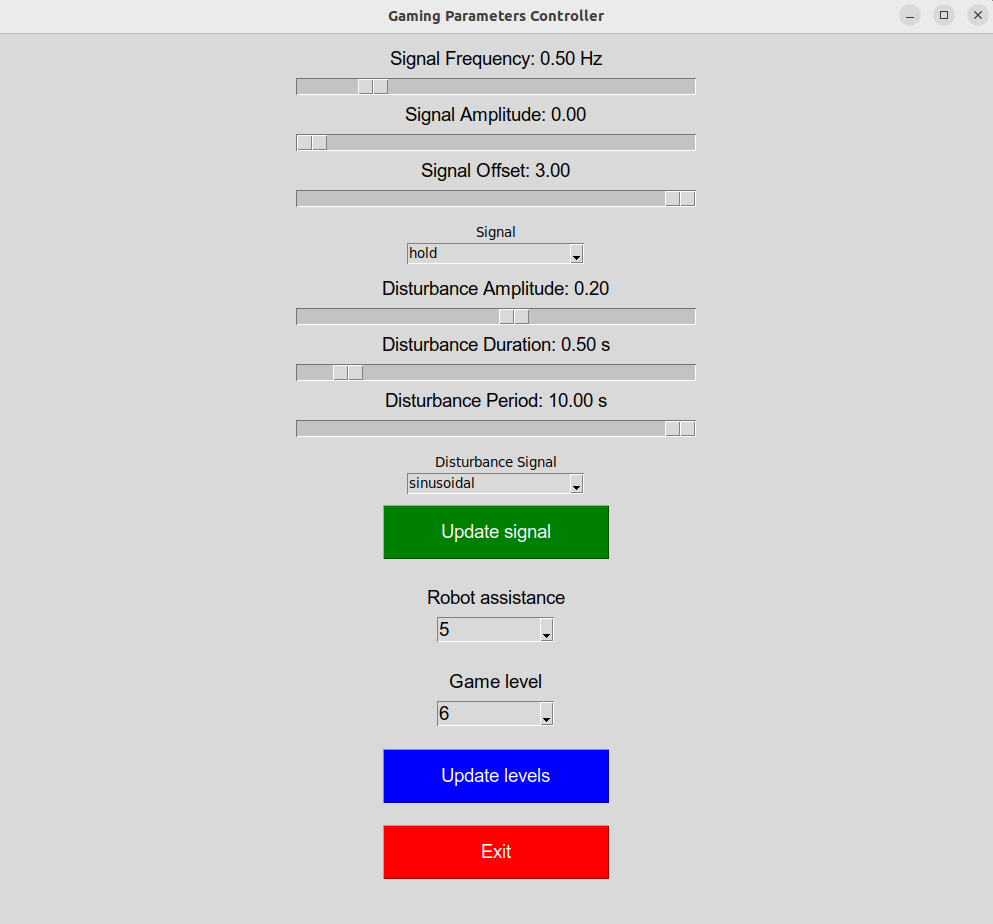
\includegraphics[width=\linewidth]{figs/control_pannel.png}
	\end{minipage}
	\caption[Interfaz de control]{Interfaz de control}
	\label{fig:control}
\end{figure}

\section{Interfaz de visualización}

Este script permite observar el comportamiento del paciente a lo largo de la terapia en un entorno gamificado.

En un principio, se mostrará una pantalla negra y un mensaje indicando que está en estado de espera hasta que un paciente comience el juego.
Una vez haya un jugador activo, el médico podrá ver una pantalla con dos gráficas.
La primera mostrará la señal de referencia y la posición del jugador, el gráfico se actualiza en tiempo real permitiendo un seguimiento continuo del rendimiento del paciente.
La segunda grafica el error de trayectoria del paciente con respecto a la deseada, lo que permite evaluar la precisión del movimiento.

El código detecta si el jugador sale de los límites definidos por la señal principal a la que se le suma y resta un offset.
Esto permite detectar fallos de control, fatiga o pérdida de atención.
Para el cálculo del error se utiliza la Fórmula \ref{ec:ec1}.

\begin{myequation}[h]
\begin{equation}
error(t) = | y_{player}(y) - y_{reference}(t) |
\nonumber
\label{ec:ec1}
\end{equation}
\caption[Cálculo del error de trayectoria]{Cálculo del error de trayectoria}
\end{myequation} 

Al finalizar la sesión, se guardan en un archivo .csv, en un subdirectorio bajo el nombre \textit{metrics}, los datos más relevantes de la sesión, como los tiempos, la señal, la posición del jugador, el offset, errores en la trayectoria y posibles colisiones, para facilitar su análisis posterior.

En la Imagen \ref{fig:visual} se puede visualizar la retroalimentación obtenida durante la terapia.

\begin{figure}[ht!]
	\centering
	\begin{minipage}{0.85\linewidth}
		\centering
		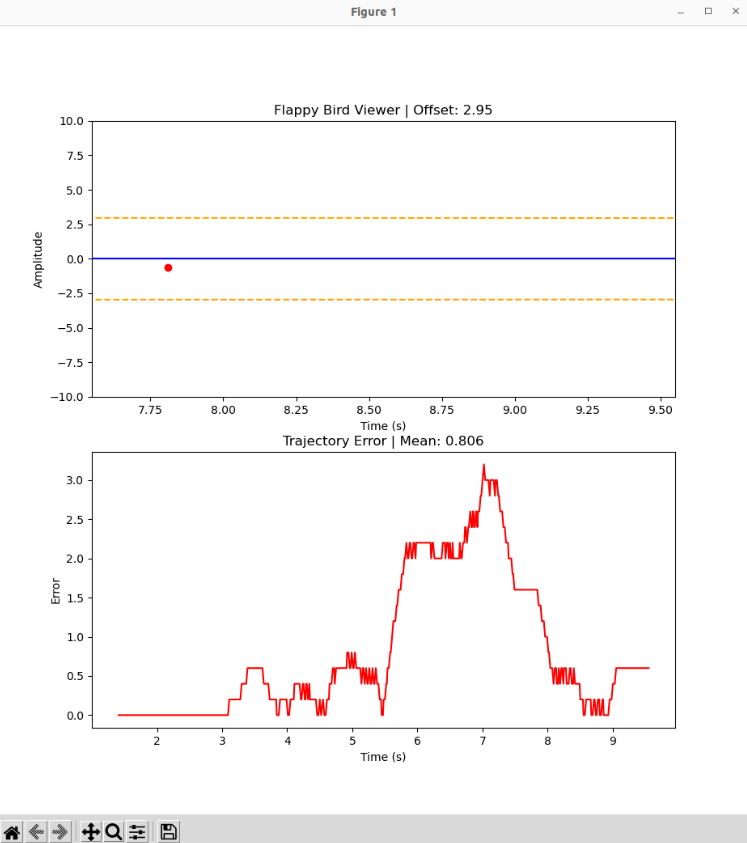
\includegraphics[width=\linewidth]{figs/visual.png}
	\end{minipage}
	\caption[Interfaz de visualización]{Interfaz de visualización}
	\label{fig:visual}
\end{figure}

\section{Juego flappy}
